
%(BEGIN_QUESTION)
% Copyright 2014, Tony R. Kuphaldt, released under the Creative Commons Attribution License (v 1.0)
% This means you may do almost anything with this work of mine, so long as you give me proper credit

Examine this schematic of a temperature control system for a steam-heated exchanger:

$$\includegraphics[width=15.5cm]{i04715x01.eps}$$

Determine the effect on the control system's regulation of temperature inside the vessel if the instrument air supply to the I/P transducer fails (i.e. goes to 0 PSI).  Assume all loop components are properly configured, that the controller is well-tuned, and that a significant amount of time has passed since the compressed air failure.  Compare these conditions with what they were before the failure:

\begin{itemize}
\item{} Control valve will: {\it open up} further, {\it close down} more, or {\it remain in the same position} 
\vskip 10pt
\item{} Process temperature will: {\it increase}, {\it decrease}, or {\it remain the same} as before
\end{itemize}

\underbar{file i04715}
%(END_QUESTION)





%(BEGIN_ANSWER)

\begin{itemize}
\item{} Control valve will: {\bf open up further}
\vskip 10pt
\item{} Process temperature will: {\bf decrease}
\end{itemize}

%(END_ANSWER)





%(BEGIN_NOTES)

{\bf This question is intended for exams only and not worksheets!}.

%(END_NOTES)

